%%%%%%%%%%%%%%%%%%%%%%%%%%%%%%%%%%%%%%%%%%%%%%%%%%%%%%%%%%%%%%%%%%%%%%%%%%%%%
%% MS Lay Summary - Pedro - 30 July 2016
%%%%%%%%%%%%%%%%%%%%%%%%%%%%%%%%%%%%%%%%%%%%%%%%%%%%%%%%%%%%%%%%%%%%%%%%%%%%%
%%%%%%%%%%%%%%%%%%%%%%%%%%%%%%%%%%%%%%%%%%%%%%%%%%%%%%%%%%%%%%%%%%%%% Headers
\documentclass[a4paper,12pt]{article}
\usepackage{geometry}
\usepackage{lscape}
\usepackage{setspace}
\usepackage{graphicx}
\usepackage{epstopdf}
\usepackage[margin=10pt,font=small,labelfont=bf]{caption}
\usepackage[left,pagewise]{lineno}
\usepackage{caption}
%%%%%%%%%%%%%%%%%%%%%%%%%%%%%%%%%%%%%%%%%%%%%%%%%%%%%%%%%%%%%%%%%% Title page
\begin{document}
\title{Lay Summary}

\author{Pedro Jordano}

%\date{Sevilla, \today}
\maketitle
\newpage
%%%%%%%%%%%%%%%%%%%%%%%%%%%%%%%%%%%%%%%%%%%%%%%%%%%%%%%%%%%%%%%%% Lay Summary
\begin{spacing}{1.5}
\section*{Seeking ecological interactions}
\subsection*{Pedro Jordano}
(245 words)\\

No species on earth lives without interacting with other species. Ecological interactions are thus a fundamental component of Biodiversity: we need to document those interactions to assess the crucial ecological services and functions that they represent.

Sampling ecological interactions presents similar challenges, problems, potential biases, and constraints as sampling individuals and species in biodiversity inventories. Robust estimates of the actual number of interactions (links) among free-living species within diversified ecological networks require adequate sampling effort that needs to be explicitly gauged, yet we still lack a sampling theory explicitly focusing on ecological interactions. Adequately assessing the completeness of a network of ecological interactions thus needs knowledge of the natural history details embedded, so that forbidden links (i.e., life-history restrictions impeding interactions) can be accounted for when addressing sampling effort. Here I outline a conceptual framework for sampling ecological interactions by building an explicit analogue to individuals and species sampling, thus extending diversity--monitoring approaches to the characterization of complex networks of ecological interactions. 

Contrary to species inventories, a sizable fraction of non-observed pairwise interactions cannot be sampled, due to biological constraints that forbid their occurrence. Recent implementations of inference methods for unobserved species or for individual--based data can be combined with the assessment of forbidden links. This is crucial to assess the rapid and devastating effects of defaunation-driven loss of key ecological interactions, and the services they provide, and the analogous losses related to interaction gains due to invasive species and biotic homogenization.

\end{spacing}
%%%%%%%%%%%%%%%%%%%%%%%%%%%%%%%%%%%%%%%%%%%%%%%%%%%%%%%%%%%%%%%%%%%%% FIGURES
%\newpage
%------------------------------------------------------------------- Figure 1
\begin{figure}
  \makebox[\textwidth][c]{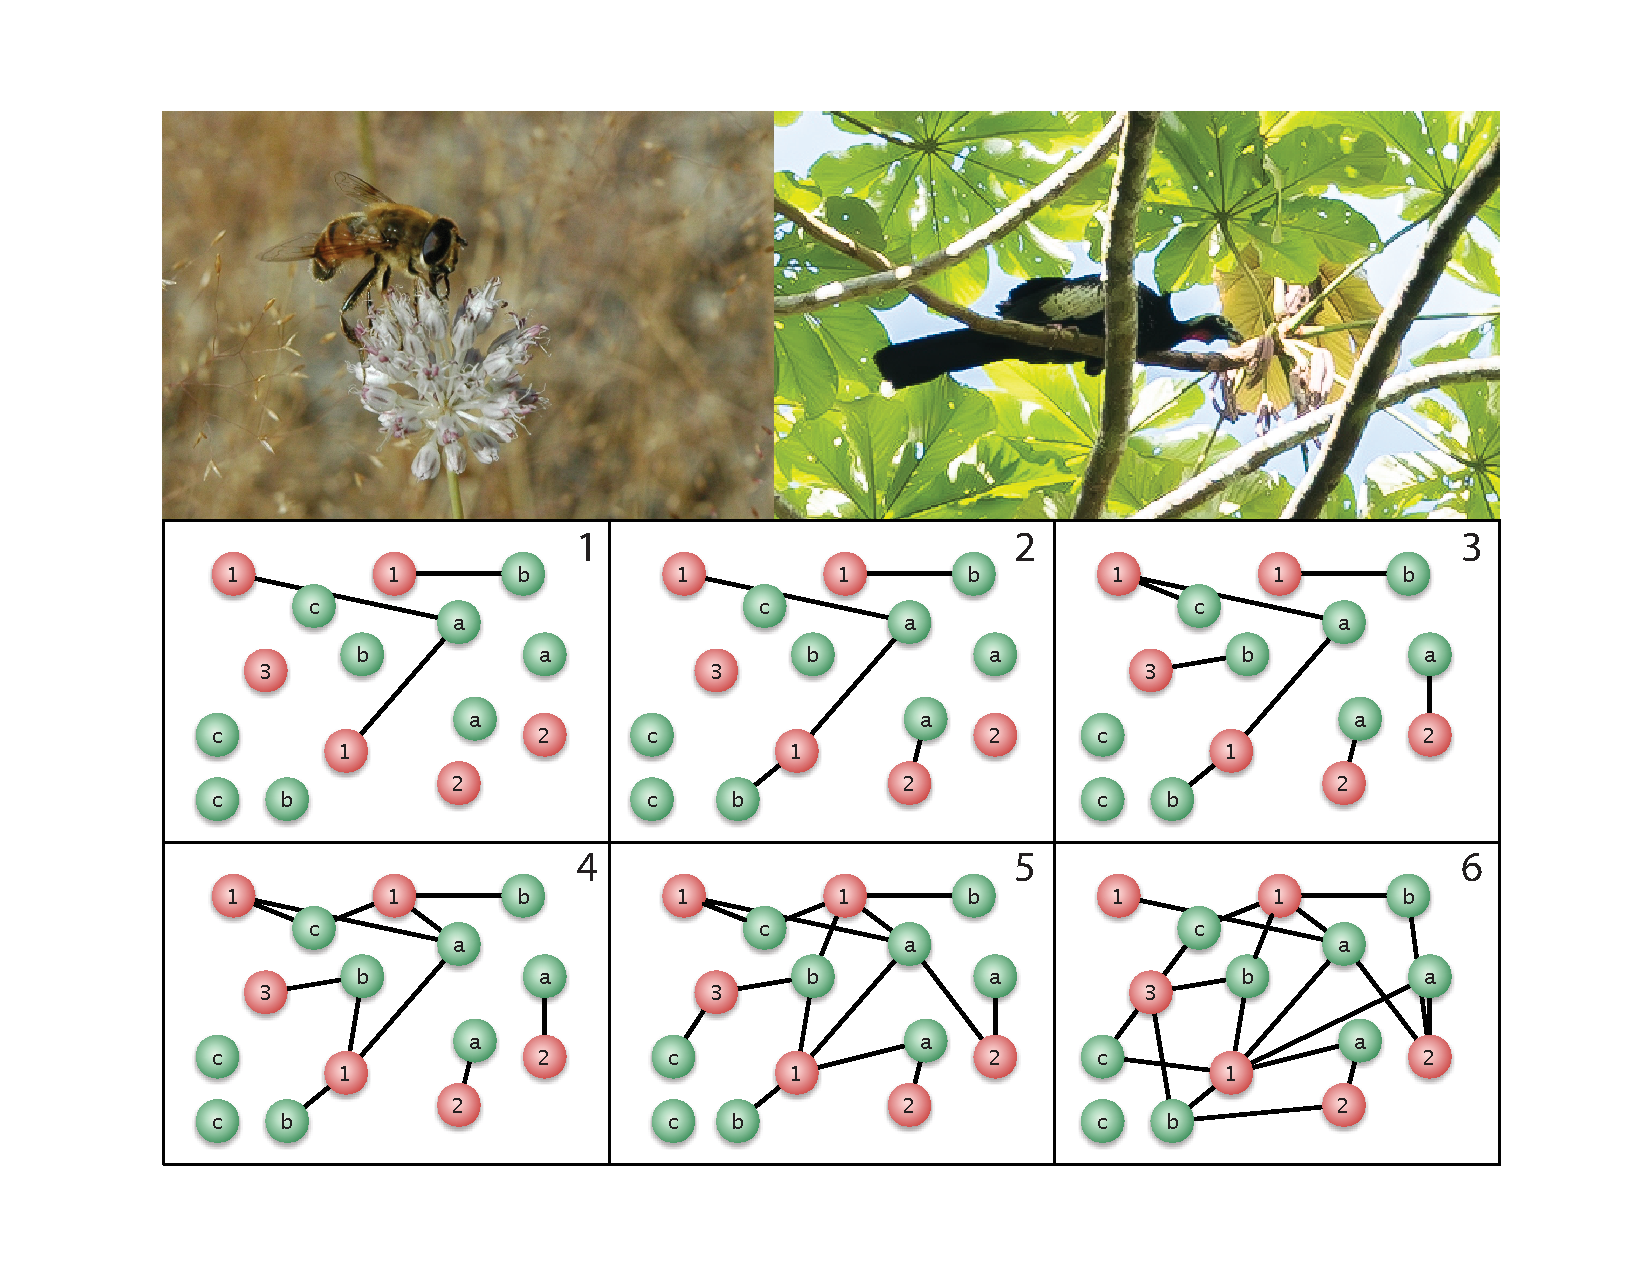
\includegraphics[width=1.5\textwidth]{Fig_laysumm.pdf}}%
  \caption{Image caption: Common Drone fly \textit{Eristalix tenax} (Syrphidae) visiting an \textit{Allium ampeloprasum} sp. (Liliaceae) (wild garlic) inflorescence in SE Spain (left), and a Jacutinga \textit{Aburria jacutinga} (Cracidae) feeding on fruits (catkins) of Red cecropia \textit{Cecropia glaziovii} (Cecropiaceae) in the Brazilan Atlantic rainforest. These are examples of pairwise interactions among individuals of plants and animals that we routinely record in the field to build network representations of the interaction patterns. We need these road--maps of mutual dependencies among species to understand the architecture that supports biodiversity. Bottom: the sampling of interactions is a cumulative process where we inventory plant-animal encounters to progressively add samples with new interactions (steps 1 to 6) that were previously undetected. This paper discusses how to estimate sampling robustness when assessing complex networks of interactions among free-living species, i.e., to what extent our study would have catalogued all the distinct pairwise interactions actually occurring. – Photos: Pedro Jordano.}
  \label{Fig_laysumm}
\end{figure}
%----------------------------------------------------------------------------
%%%%%%%%%%%%%%%%%%%%%%%%%%%%%%%%%%%%%%%%%%%%%%%%%%%%%%%%%%%%%%%%%%%%%%%%%%%%%
\end{document}

